\documentclass[dvisvgm]{standalone}
\usepackage{tikz}
\usepackage{pgfplots}
\usepackage{amsmath}
\usepackage{amssymb}

\pgfplotsset{compat=1.18}

\begin{document}
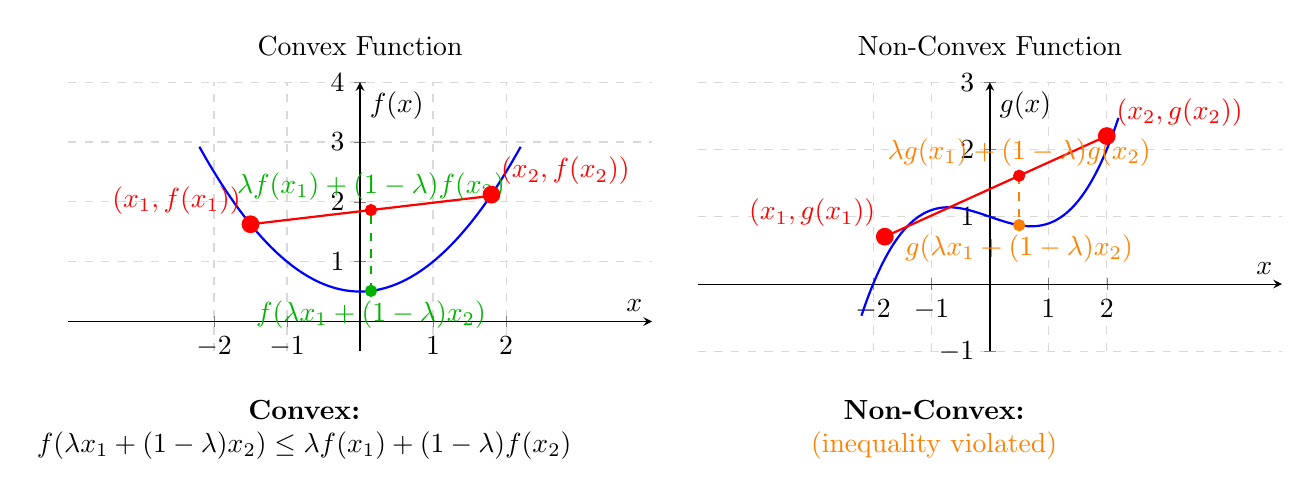
\begin{tikzpicture}
    % Convex function (left side)
    \begin{scope}[xshift=0cm]
        \begin{axis}[
            width=9cm,
            height=5cm,
            axis lines=middle,
            xlabel={$x$},
            ylabel={$f(x)$},
            title={Convex Function},
            xmin=-4, xmax=4,
            ymin=-0.5, ymax=4,
            xtick={-2,-1,0,1,2},
            ytick={0,1,2,3,4},
            grid=major,
            grid style={dashed, gray!30},
        ]
        
        % Plot convex function f(x) = 0.5x^2 + 0.5
        \addplot[blue, thick, domain=-2.2:2.2, samples=100] {0.5*x^2 + 0.5};
        
        % Define points: x1=-1.5, f(x1)=1.625; x2=1.8, f(x2)=2.12
        % Chord equation: y = 0.144x + 1.841
        \addplot[red, thick, domain=-1.5:1.8] {0.144*x + 1.841};
        
        % Draw points
        \addplot[only marks, mark=*, mark size=3pt, red] coordinates {(-1.5, 1.625) (1.8, 2.12)};
        
        % Labels for points
        \node[above left, red] at (-1.5, 1.625) {$(x_1, f(x_1))$};
        \node[above right, red] at (1.8, 2.12) {$(x_2, f(x_2))$};
        
        % Mark a point on function and chord for comparison (x=0.15)
        \addplot[only marks, mark=*, mark size=2pt, green!70!black] coordinates {(0.15, 0.511)};
        \addplot[only marks, mark=*, mark size=2pt, red] coordinates {(0.15, 1.862)};
        
        % Draw vertical line showing inequality
        \draw[dashed, green!70!black, thick] (0.15, 0.511) -- (0.15, 1.862);
        
        \node[below, green!70!black] at (0.15, 0.511) {$f(\lambda x_1 + (1-\lambda)x_2)$};
        \node[above, green!70!black] at (0.15, 1.862) {$\lambda f(x_1) + (1-\lambda)f(x_2)$};
        
        \end{axis}
        
        % Convexity inequality text
        \node[align=center, below] at (3, -0.5) {
            \textbf{Convex:} \\
            $f(\lambda x_1 + (1-\lambda)x_2) \leq \lambda f(x_1) + (1-\lambda)f(x_2)$
        };
    \end{scope}
    
    % Non-convex function (right side)
    \begin{scope}[xshift=8cm]
        \begin{axis}[
            width=9cm,
            height=5cm,
            axis lines=middle,
            xlabel={$x$},
            ylabel={$g(x)$},
            title={Non-Convex Function},
            xmin=-5, xmax=5,
            ymin=-1, ymax=3,
            xtick={-2,-1,0,1,2},
            ytick={-1,0,1,2,3},
            grid=major,
            grid style={dashed, gray!30},
        ]
        
        % Plot non-convex function g(x) = 0.2x^3 - 0.3x + 1
        \addplot[blue, thick, domain=-2.2:2.2, samples=100] {0.2*x^3 - 0.3*x + 1};
        
        % Define points: x1=-1.8, g(x1)=0.704; x2=2.0, g(x2)=2.2
        % Chord equation: y = 0.394x + 1.413
        \addplot[red, thick, domain=-1.8:2.0] {0.394*x + 1.413};
        
        % Draw points
        \addplot[only marks, mark=*, mark size=3pt, red] coordinates {(-1.8, 0.704) (2.0, 2.2)};
        
        % Labels for points
        \node[above left, red] at (-1.8, 0.704) {$(x_1, g(x_1))$};
        \node[above right, red] at (2.0, 2.2) {$(x_2, g(x_2))$};
        
        % Mark a point where function is above the chord (x=0.5)
        \addplot[only marks, mark=*, mark size=2pt, orange] coordinates {(0.5, 0.875)};
        \addplot[only marks, mark=*, mark size=2pt, red] coordinates {(0.5, 1.610)};
        
        % Draw vertical line showing violation of inequality
        \draw[dashed, orange, thick] (0.5, 1.610) -- (0.5, 0.875);
        
        \node[below, orange] at (0.5, 0.875) {$g(\lambda x_1 + (1-\lambda)x_2)$};
        \node[above, orange] at (0.5, 1.610) {$\lambda g(x_1) + (1-\lambda)g(x_2)$};
        
        \end{axis}
        
        % Non-convexity inequality text
        \node[align=center, below] at (3, -0.5) {
            \textbf{Non-Convex:} \\
            \textcolor{orange}{(inequality violated)}
        };
    \end{scope}
    
    
\end{tikzpicture}
\end{document}
